\subsection{Sao lưu và khôi phục khóa bí mật phiếu}

Sau khi bỏ phiếu, cử tri giữ một tập \textit{khóa bí mật phiếu} ngay trên thiết bị di động — gồm các hệ số làm mù $(\alpha, \beta)$, hai thành phần chữ ký $(h, s')$ và danh sách ứng viên đã chọn — được lưu trong kho lưu trữ an toàn (\textit{Secure Store}) của hệ điều hành. Tập khóa này là điều kiện bắt buộc để cử tri tiết lộ phiếu và tự xác minh phiếu về sau; mất thiết bị đồng nghĩa mất vĩnh viễn khả năng đó. Hệ thống vì vậy cung cấp cơ chế sao lưu và khôi phục các khóa này lên máy chủ mà vẫn không làm suy giảm tính bí mật, theo mô hình \textit{zero-knowledge}.

\subsubsection{Lớp mã hóa phía máy khách (zero-knowledge)}

Toàn bộ việc mã hóa diễn ra trên thiết bị, trước khi bất kỳ dữ liệu nào rời khỏi máy khách. Cử tri đặt một mã PIN; ứng dụng dẫn xuất khóa đối xứng 256-bit từ mã PIN bằng hàm \pkg{PBKDF2-SHA256} với $100{,}000$ vòng lặp và một salt ngẫu nhiên, sau đó mã hóa tập khóa bằng \pkg{AES-256-GCM}. Kết quả là một gói dữ liệu (\textit{envelope}) JSON chứa tham số dẫn xuất khóa (thuật toán, số vòng, salt) và phần bản mã (vector khởi tạo, bản mã kèm thẻ xác thực). Vì máy chủ \textbf{không bao giờ nhận mã PIN}, máy chủ không thể dẫn lại khóa nên không thể giải lớp mã hóa này. Số vòng lặp lớn của PBKDF2 làm chậm đáng kể tấn công dò mã PIN theo kiểu vét cạn. Hình~\ref{fig:backup-derive-key} trình bày hàm dẫn xuất khóa và mã hóa gói envelope.

\begin{figure}[H]
    \centering
    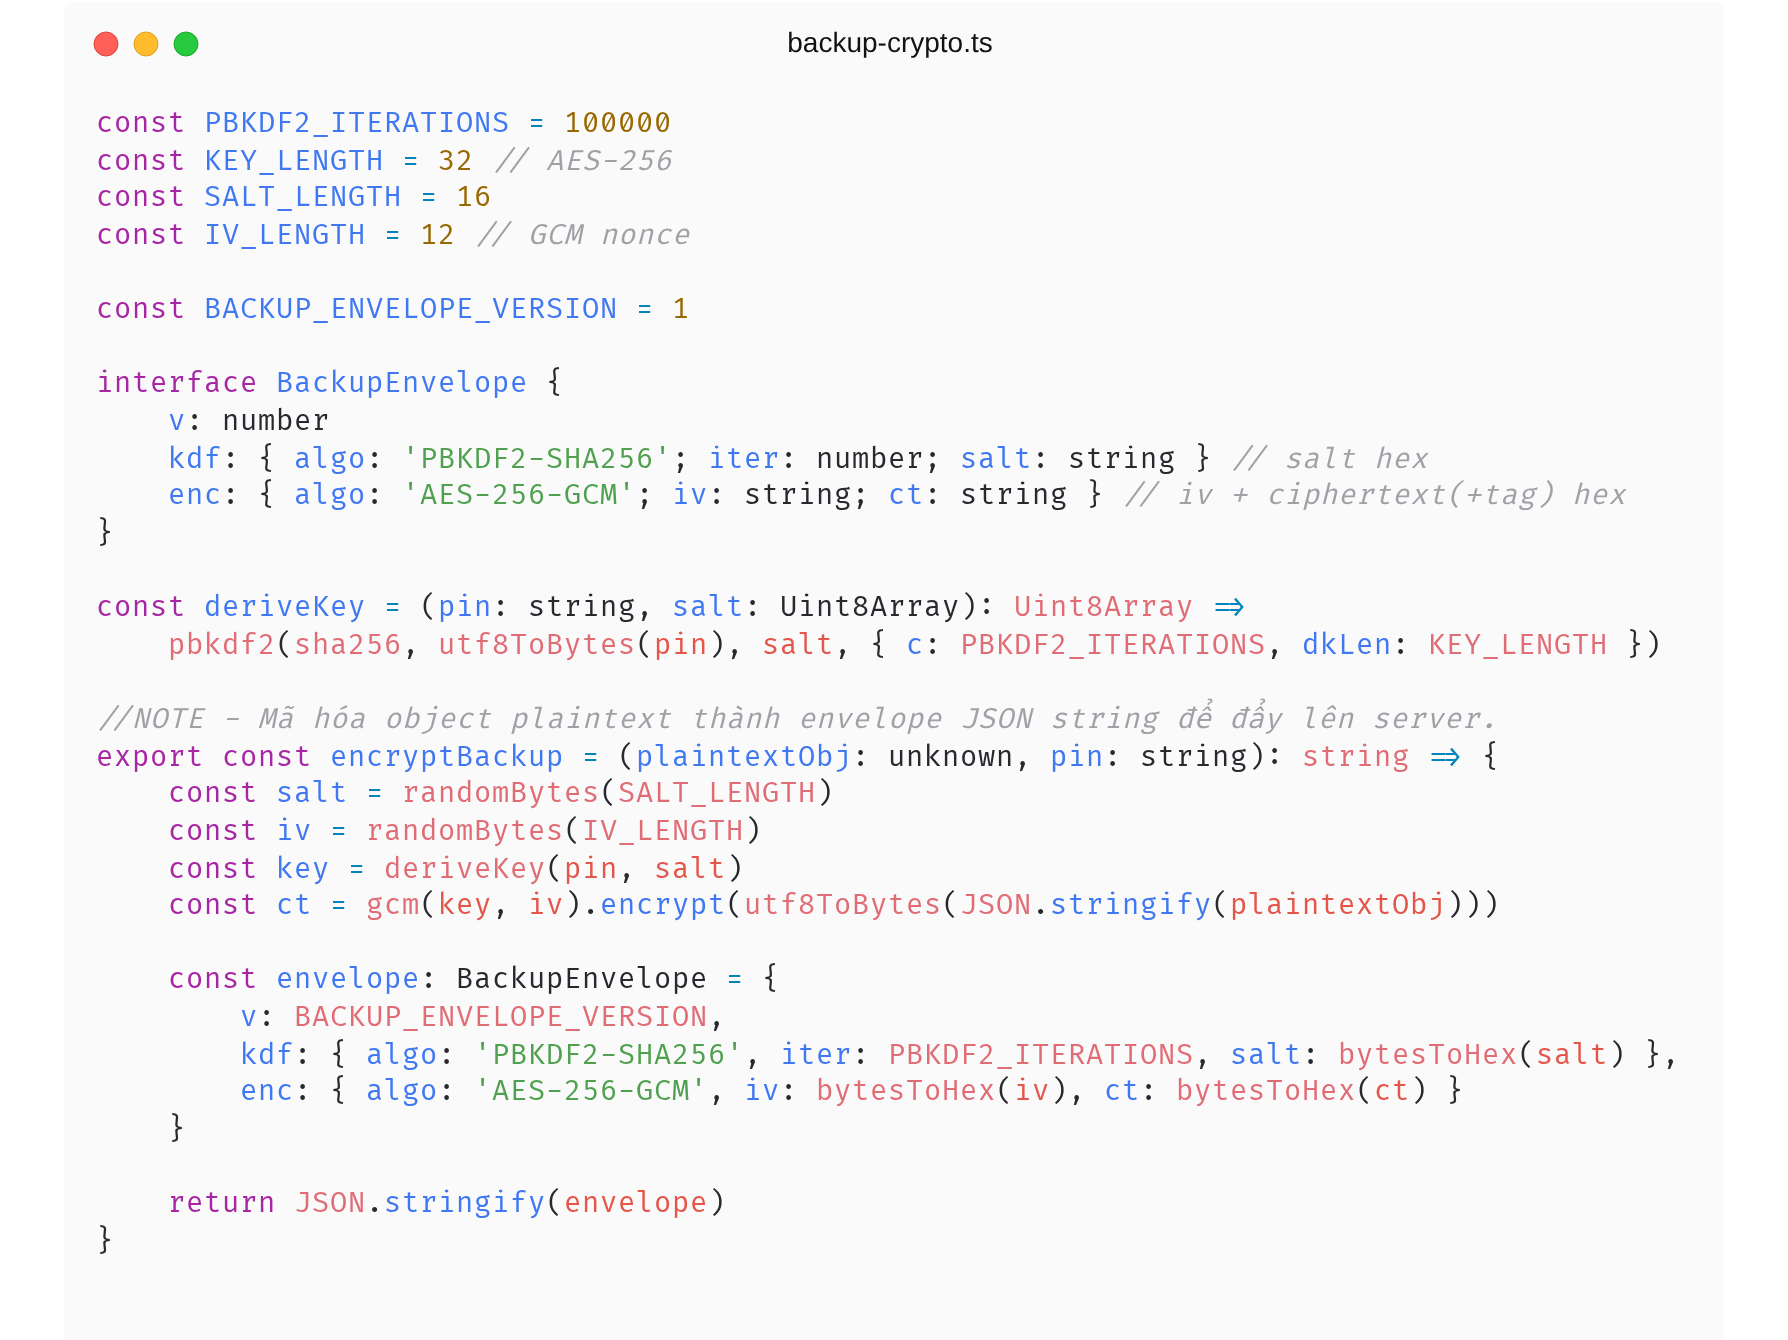
\includegraphics[width=\textwidth, keepaspectratio]{Figures/code/backup-derive-key.png}
    \caption{Hàm dẫn xuất khóa từ mã PIN bằng PBKDF2-SHA256 và mã hóa gói sao lưu bằng AES-256-GCM phía máy khách}
    \label{fig:backup-derive-key}
\end{figure}

\subsubsection{Lớp mã hóa dữ liệu khi lưu trữ (\textit{at-rest encryption}) phía máy chủ}

Khi nhận được gói envelope, Identity Service áp dụng thêm \textbf{một lớp mã hóa thứ hai} trước khi ghi xuống MongoDB nhằm bảo vệ dữ liệu khi lưu trữ. Lớp này dẫn xuất khóa bằng \pkg{argon2id} từ một bí mật phía máy chủ \pkg{BACKUP\_SECRET} kết hợp một salt ngẫu nhiên theo từng bản ghi, rồi mã hóa bằng \pkg{AES-256-GCM}. Như vậy, một bản sao lưu chịu hai lớp mã hóa độc lập: lớp ngoài chỉ giải được bằng mã PIN của cử tri, lớp trong chỉ giải được khi máy chủ nắm \pkg{BACKUP\_SECRET}. Kẻ tấn công đọc trộm cơ sở dữ liệu sẽ không thu được gì nếu thiếu cả hai bí mật này.

\subsubsection{Khôi phục và lưu ý vận hành}

Khi khôi phục, Identity Service gỡ lớp mã hóa dữ liệu khi lưu trữ và trả lại gói envelope nguyên bản do máy khách tạo; ứng dụng dẫn lại khóa từ mã PIN và giải mã. Nhờ \pkg{AES-256-GCM} là mã hóa có xác thực (\textit{authenticated encryption}), một mã PIN sai sẽ khiến bước kiểm tra thẻ xác thực thất bại ngay tại máy khách và ứng dụng báo lỗi ``Mã PIN không đúng'' — máy chủ không tham gia và cũng không học được bất kỳ thông tin nào về mã PIN.

Về vận hành, biến môi trường \pkg{BACKUP\_SECRET} của Identity Service phải được đặt bằng một giá trị mạnh trong môi trường sản xuất; giá trị mặc định dự phòng chỉ phục vụ phát triển cục bộ. Lý tưởng nhất, bí mật này nên được quản lý bởi một kho bí mật chuyên dụng thay vì lưu trong tệp cấu hình.
